\section{ResNet}
\subsection{Resnet là gì}
ResNet (Residual Network) được giới thiệu đến công chúng vào năm 2015 và thậm chí đã giành được vị trí thứ 1 trong cuộc thi ILSVRC 2015 với tỉ lệ lỗi top 5 chỉ 3.57\%. Không những thế nó còn đứng vị trí đầu tiên trong cuộc thi ILSVRC and COCO 2015 với ImageNet Detection, ImageNet localization, Coco detection và Coco segmentation.Hiện tại thì có rất nhiều biến thể của kiến trúc ResNet với số lớp khác nhau như ResNet-18, ResNet-34, ResNet-50, ResNet-101, ResNet-152,...Với tên là ResNet theo sau là một số chỉ kiến trúc ResNet với số lớp nhất định.

Các kiến trúc mạng trước khi Resnet ra đời như Alexnet, VGG được coi là các mạng nơ ron thuần (plain network). Đối với các mạng nơ ron thuần, Kaiming He\cite{resnet} đã thí nghiệm và đưa ra kết luận khi tăng số lượng layer của mạng từ 20 lên 56 thì lỗi trên tập huấn luyện và trên tập kiểm tra của mạng 56 layer đều cao hơn so với mạng 20 layer(hình \ref{fig:resnet_vanishing_gradient}). 
\begin{figure}[H]
	\centering
	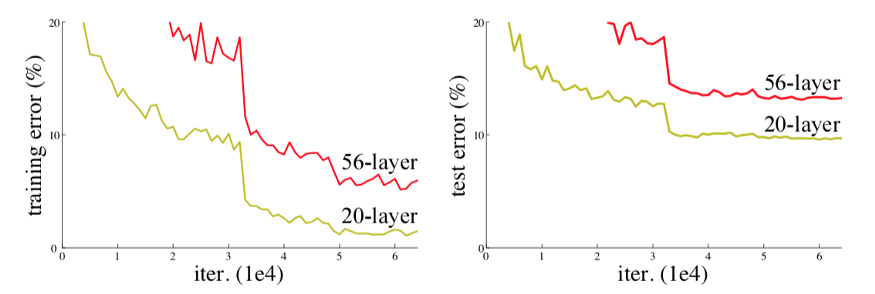
\includegraphics[width=1\linewidth]{images/resnet_vanishing_gradient}
	\caption{Lỗi huấn luyện và lỗi kiểm tra với mạng 20 layer và 56 layer.}
	\label{fig:resnet_vanishing_gradient}
\end{figure} 
ResNet đưa ra là sử dụng kết nối "tắt" đồng nhất để xuyên qua một hay nhiều lớp. Một khối như vậy được gọi là một Residual Block(hình \ref{fig:resnet_residual_block}). Ý tưởng chính của phương pháp này thực ra rất đơn giản, Resnet thực hiện residual mapping để copy thông tin từ các layer nông shallow layer trước đó đến các layer sâu hơn. Chúng ta giả sử output của shallow layer là $x$. Trong quá trình forward của mạng nó được đưa qua một phép biến đổi tuyến tính $F(x)$. Chúng ta giả sử output của phép biến đổi tuyền tính này là $H(x)$. Một residual (phần dư) giữa deep layer và shallow layer là
$$\mathcal{F}(\mathbf{x}; W_i) := \mathcal{H}(\mathbf{x}) - \mathbf{x}$$
Trong đó, $W_i$ là các tham số của mô hình CNN với phép biến đổi $F$ và nó được tối ưu trong quá trình huấn luyện.
\begin{figure}[H]
	\centering
	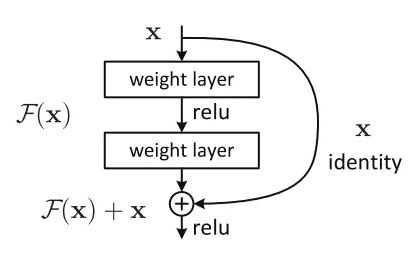
\includegraphics[width=0.5\linewidth]{images/resnet_residual_block}
	\caption{Residual block.}
	\label{fig:resnet_residual_block}
\end{figure}
Việc thêm vào các residual block vào trong kiến trúc mạng deep learning có hai cách tuỳ thuộc vào từng trường hợp cụ thể.
\begin{itemize}
	\item {\bf identity mapping} trong trường hợp này residual mapping đơn giản là việc cộng trực tiếp $x$ vào đầu ra của các stacked block $F(x)$. Đây là một cách sử dụng khá phổ biến trong thiết kế mạng ResNet nếu như input activation có cùng số chiều với output activation.
	\begin{figure}[H]
		\centering
		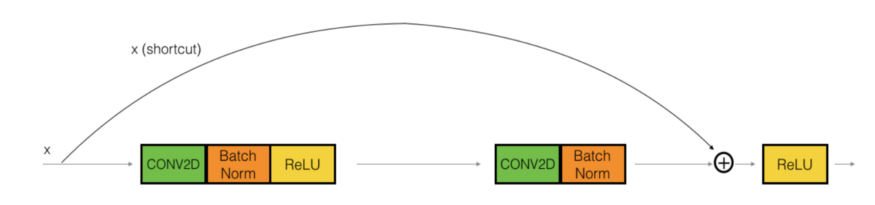
\includegraphics[width=1\linewidth]{images/resnet_identity_mapping}
		\caption{Identity mapping.}
		\label{fig:resnet_identity_mapping}
	\end{figure}
	\item {\bf Convolutional block} một trường hợp khác là thay vì cộng trực tiếp giá trị của input activation chúng ta sẽ đưa qua một convolution transformation. Trường hợp này có thể được thực hiện trong trường hợp input activation và output activation có số chiều khác nhau. Lúc này đầu ra được xác định như sau $y=F(x;Wi)+\text{Conv}(x)$.
	\begin{figure}[H]
		\centering
		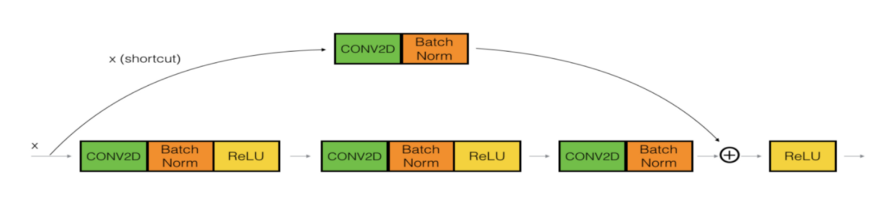
\includegraphics[width=1\linewidth]{images/resnet_conv_block}
		\caption{Convolutional block.}
		\label{fig:resnet_conv_block}
	\end{figure}
\end{itemize}
\subsection{Kiến trúc của Resnet}
Hình \ref{fig:resnet_architecture} dưới đây mô tả chi tiết kiến trúc mạng nơ ron ResNet
\begin{figure}[H]
	\centering
	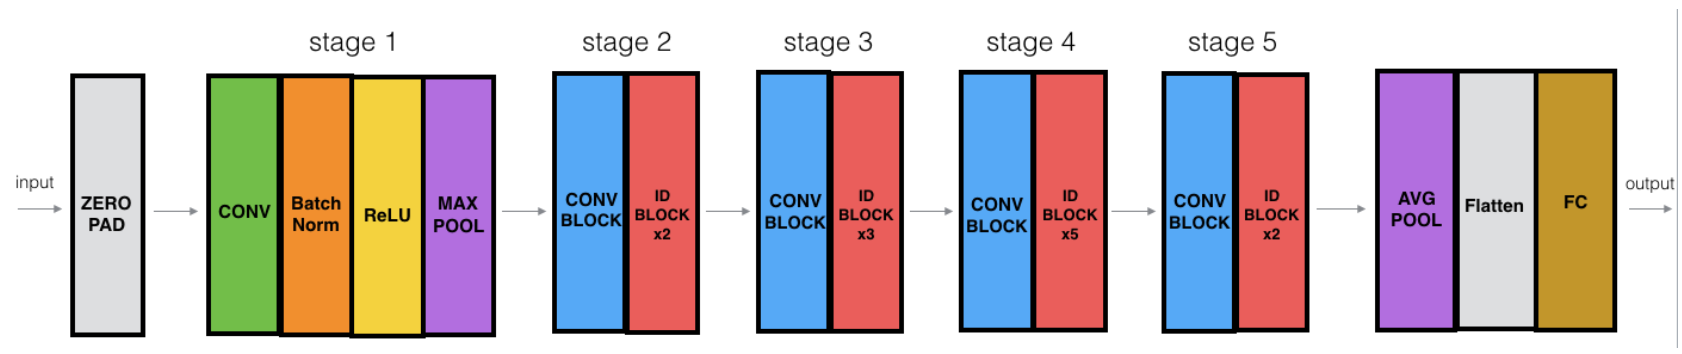
\includegraphics[width=1\linewidth]{images/resnet_architecture}
	\caption{Kiến trúc mạng ResNet.}
	\label{fig:resnet_architecture}
\end{figure}
"ID BLOCK" trong hình trên là viết tắt của từ Identity block và ID BLOCK x3 nghĩa là có 3 khối Identity block chồng lên nhau. Nội dung hình \ref{fig:resnet_architecture} như sau:
\begin{itemize}
	\item Zero-padding : Input với (3,3)
	\item Stage 1 : Tích chập (Conv1) với 64 filters với shape(7,7), sử dụng stride (2,2). BatchNorm, MaxPooling (3,3).
	\item Stage 2 : Convolutiontal block sử dụng 3 filter với size 64x64x256, f=3, s=1. Có 2 Identity blocks với filter size 64x64x256, f=3.
	\item Stage 3 : Convolutional sử dụng 3 filter size 128x128x512, f=3,s=2. Có 3 Identity blocks với filter size 128x128x512, f=3.
	\item Stage 4 : Convolutional sử dụng 3 filter size 256x256x1024, f=3,s=2. Có 5 Identity blocks với filter size 256x256x1024, f=3.
	\item Stage 5 :Convolutional sử dụng 3 filter size 512x512x2048, f=3,s=2. Có 2 Identity blocks với filter size 512x512x2048, f=3.
	\item The 2D Average Pooling : sử dụng với kích thước (2,2).
	\item The Flatten.
	\item Fully Connected (Dense) : sử dụng softmax activation.
\end{itemize}

\subsection{Cài đặt Resnet}
\begin{lstlisting}[language=Python]
def ResNet50(input_shape = (512, 512, 1), classes = 2):

	# Define the input as a tensor with shape input_shape
	X_input = Input(input_shape)
	
	
	# Zero-Padding
	X = ZeroPadding2D((3, 3))(X_input)
	
	# Stage 1
	X = Conv2D(64, (7, 7), strides = (2, 2), name = 'conv1', kernel_initializer = glorot_uniform(seed=0))(X)
	X = BatchNormalization(axis = 3, name = 'bn_conv1')(X)
	X = Activation('relu')(X)
	X = MaxPooling2D((3, 3), strides=(2, 2))(X)
	
	# Stage 2
	X = convolutional_block(X, f = 3, filters = [64, 64, 256], stage = 2, block='a', s = 1)
	X = identity_block(X, 3, [64, 64, 256], stage=2, block='b')
	X = identity_block(X, 3, [64, 64, 256], stage=2, block='c')
	
	
	# Stage 3 
	X = convolutional_block(X, f = 3, filters = [128, 128, 512], stage = 3, block='a', s = 2)
	X = identity_block(X, 3, [128, 128, 512], stage=3, block='b')
	X = identity_block(X, 3, [128, 128, 512], stage=3, block='c')
	X = identity_block(X, 3, [128, 128, 512], stage=3, block='d')
	
	# Stage 4 
	X = convolutional_block(X, f = 3, filters = [256, 256, 1024], stage = 4, block='a', s = 2)
	X = identity_block(X, 3, [256, 256, 1024], stage=4, block='b')
	X = identity_block(X, 3, [256, 256, 1024], stage=4, block='c')
	X = identity_block(X, 3, [256, 256, 1024], stage=4, block='d')
	X = identity_block(X, 3, [256, 256, 1024], stage=4, block='e')
	X = identity_block(X, 3, [256, 256, 1024], stage=4, block='f')
	
	# Stage 5 
	X = convolutional_block(X, f = 3, filters = [512, 512, 2048], stage = 5, block='a', s = 2)
	X = identity_block(X, 3, [512, 512, 2048], stage=5, block='b')
	X = identity_block(X, 3, [512, 512, 2048], stage=5, block='c')
	
	# AVGPOOL . Use "X = AveragePooling2D(...)(X)"
	X = AveragePooling2D()(X)
	
	# output layer
	X = Flatten()(X)
	X = Dense(classes, activation='softmax', name='fc' + str(classes), kernel_initializer = glorot_uniform(seed=0))(X)
	
	
	# Create model
	model = Model(inputs = X_input, outputs = X, name='ResNet50')
	
	return model
\end{lstlisting}

\subsection{Ưu nhược điểm của ResNet}
\textbf{Ưu điểm:}
\begin{itemize}
	\item Kiến trúc ResNet không cần phải kích hoạt tất cả các nơ-ron trong mọi epoch (một epoch được tính là khi chúng ta đưa tất cả dữ liệu trong tập train vào mạng neural network 1 lần). Điều này làm giảm đáng kể thời gian đào tạo và cải thiện độ chính xác. Khi một đặc trưng đã được học, nó sẽ không cố gắng học lại mà tập trung vào việc học các đặc trưng mới hơn. Một cách tiếp cận rất thông minh đã cải thiện đáng kể hiệu suất đào tạo mô hình.
	\item ResNets giải quyết được khá tốt vấn đề Vanishing Gradient của các mạng CNN thuần.
	\item Có thể đào tạo dễ dàng các mạng với số lớp rất lớn mà không làm tăng tỷ lệ đào tạo lỗi.
\end{itemize}
\textbf{Nhược điểm: \cite{resnet_disadvantage}}
\begin{itemize}
	\item Đối với mạng sâu hơn, việc phát hiện lỗi trở nên khó khăn.
	\item Nếu mạng quá nông, việc đào tạo có thể rất kém hiệu quả.
\end{itemize}